\chapter{دانلود اوبونتو}
اوبونتو سیستم‌عاملی آزاد و رایگان می‌باشد که می‌توان آن را از وب‌گاه رسمی آن به نشانی زیر دانلود نمود.

\begin{url-address}
\input{urls/ubuntu_download}
\end{url-address}
 این صفحه از وب‌گاه به صورت زیر است.
\begin{figure}[hbtp]
\centering
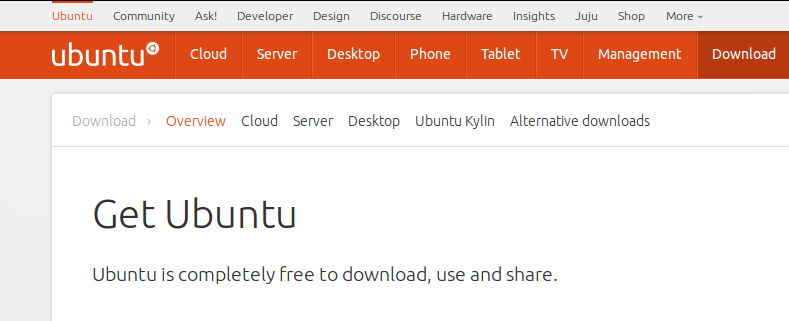
\includegraphics[scale=0.5]{pics/ubuntu-download.png}
\caption{صفحه‌ی دانلود اوبونتو}
\label{fig:ubuntu-download}
\end{figure}

همان‌طور که در عکس قابل مشاهده است، پنج گزینه برای دانلود در دسترس می‌باشد:
\begin{description}
\item[\lr{Cloud}] این ویرایش مخصوص کسانی است که می‌خواهند از اوبونتو برای محیط ابری استفاده کنند.
\item[\lr{Server}] این ویرایش مخصوص کاربرانی است که قصد ایجاد سرور بر پایه‌ی اوبونتو دارند.
\item[\lr{Desktop}] این ویرایش مخصوص کاربران خانگی و برای استفاده‌ی روزمره است.
\item[\lr{Ubuntu Kylin}] این نسخه مخصوص کاربران چینی اوبونتو است
\item[\lr{Alternative downloads}] این نسخه مخصوص کاربران چینی اوبونتو است
\end{description}